\subsection{Portas Lógicas de Redstone}

No Minecraft, a implementação de portas lógicas não depende diretamente de transistores físicos, mas sim de abstrações comportamentais do sistema de redstone.

\subsubsection{Or}

No jogo, a porta Or é a mais simples de todas, se nossas variáveis $A$ e $B$ propagam em fios opostos, para fazer uma porta Or, basta juntar estes dois fios na saida $X$, já que qualquer um deles pode energizar $X$.

\begin{figure}[H]
   	\centering
   	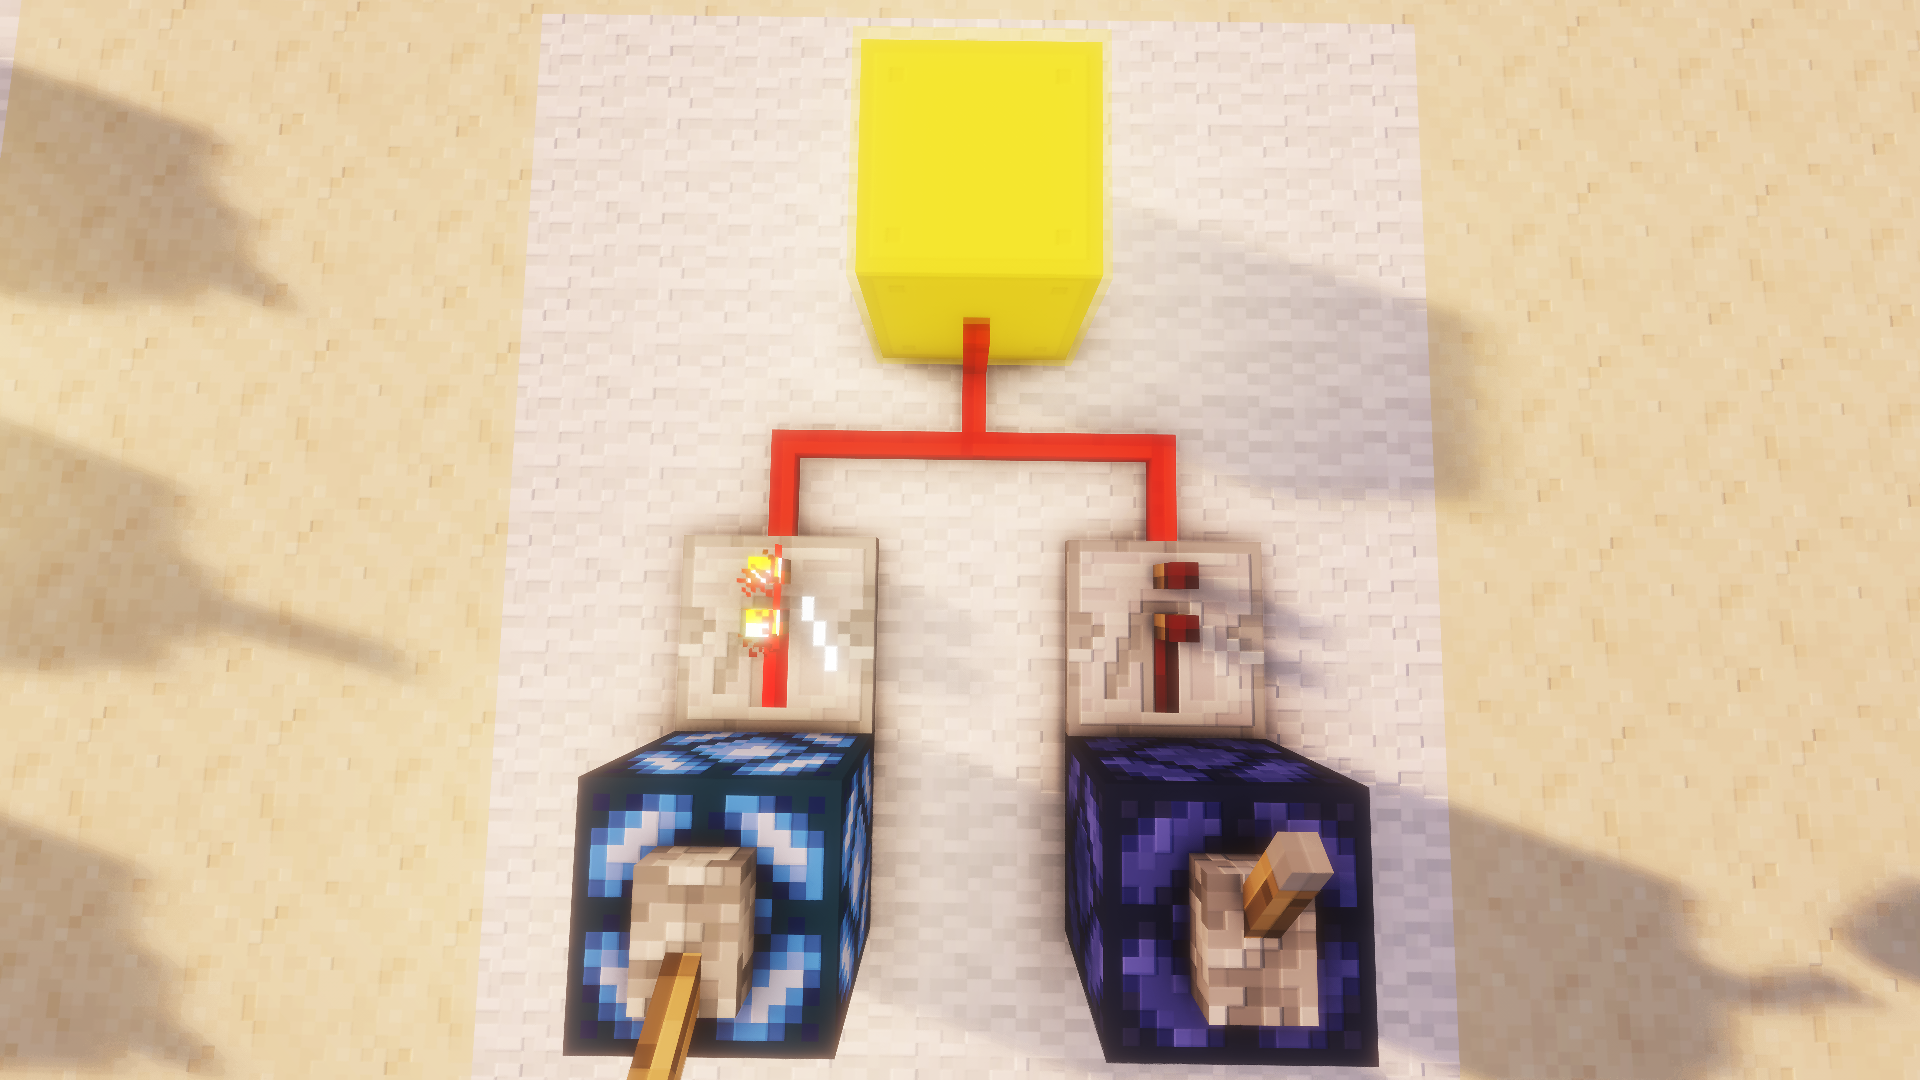
\includegraphics[width=0.7\linewidth]{images/or-redstone.png}
  	 \caption{Porta Or de Redstone}
   	\label{fig:or-redstone}
	%{\footnotesize Fonte: \url{https://autoctrls.com/datasheet-transistor/}}
\end{figure}

\subsubsection{Not}

A porta lógica NOT (ou inversor) é uma das implementações mais fundamentais em circuitos de Redstone. No Minecraft vanilla, ela é tradicionalmente construída utilizando uma tocha de redstone.

O funcionamento baseia-se no fato de que a tocha de redstone inverte o estado do sinal de entrada:
quando não há energia na entrada, a tocha permanece ligada, emitindo sinal na saída; quando a entrada é energizada, a tocha desliga, interrompendo o sinal.

\begin{figure}[H]
    \centering
    \includegraphics[width=0.7\linewidth]{images/not-redstone.png}
    \caption{Porta Not de Redstone utilizando tocha}
    \label{fig:not-redstone}
\end{figure}

Em algumas modificações do jogo (como o mod citado “Wired Redstone”), a porta NOT pode ser implementada como um componente dedicado, aumentando a eficiência espacial em circuitos complexos.

\begin{figure}[H]
    \centering
    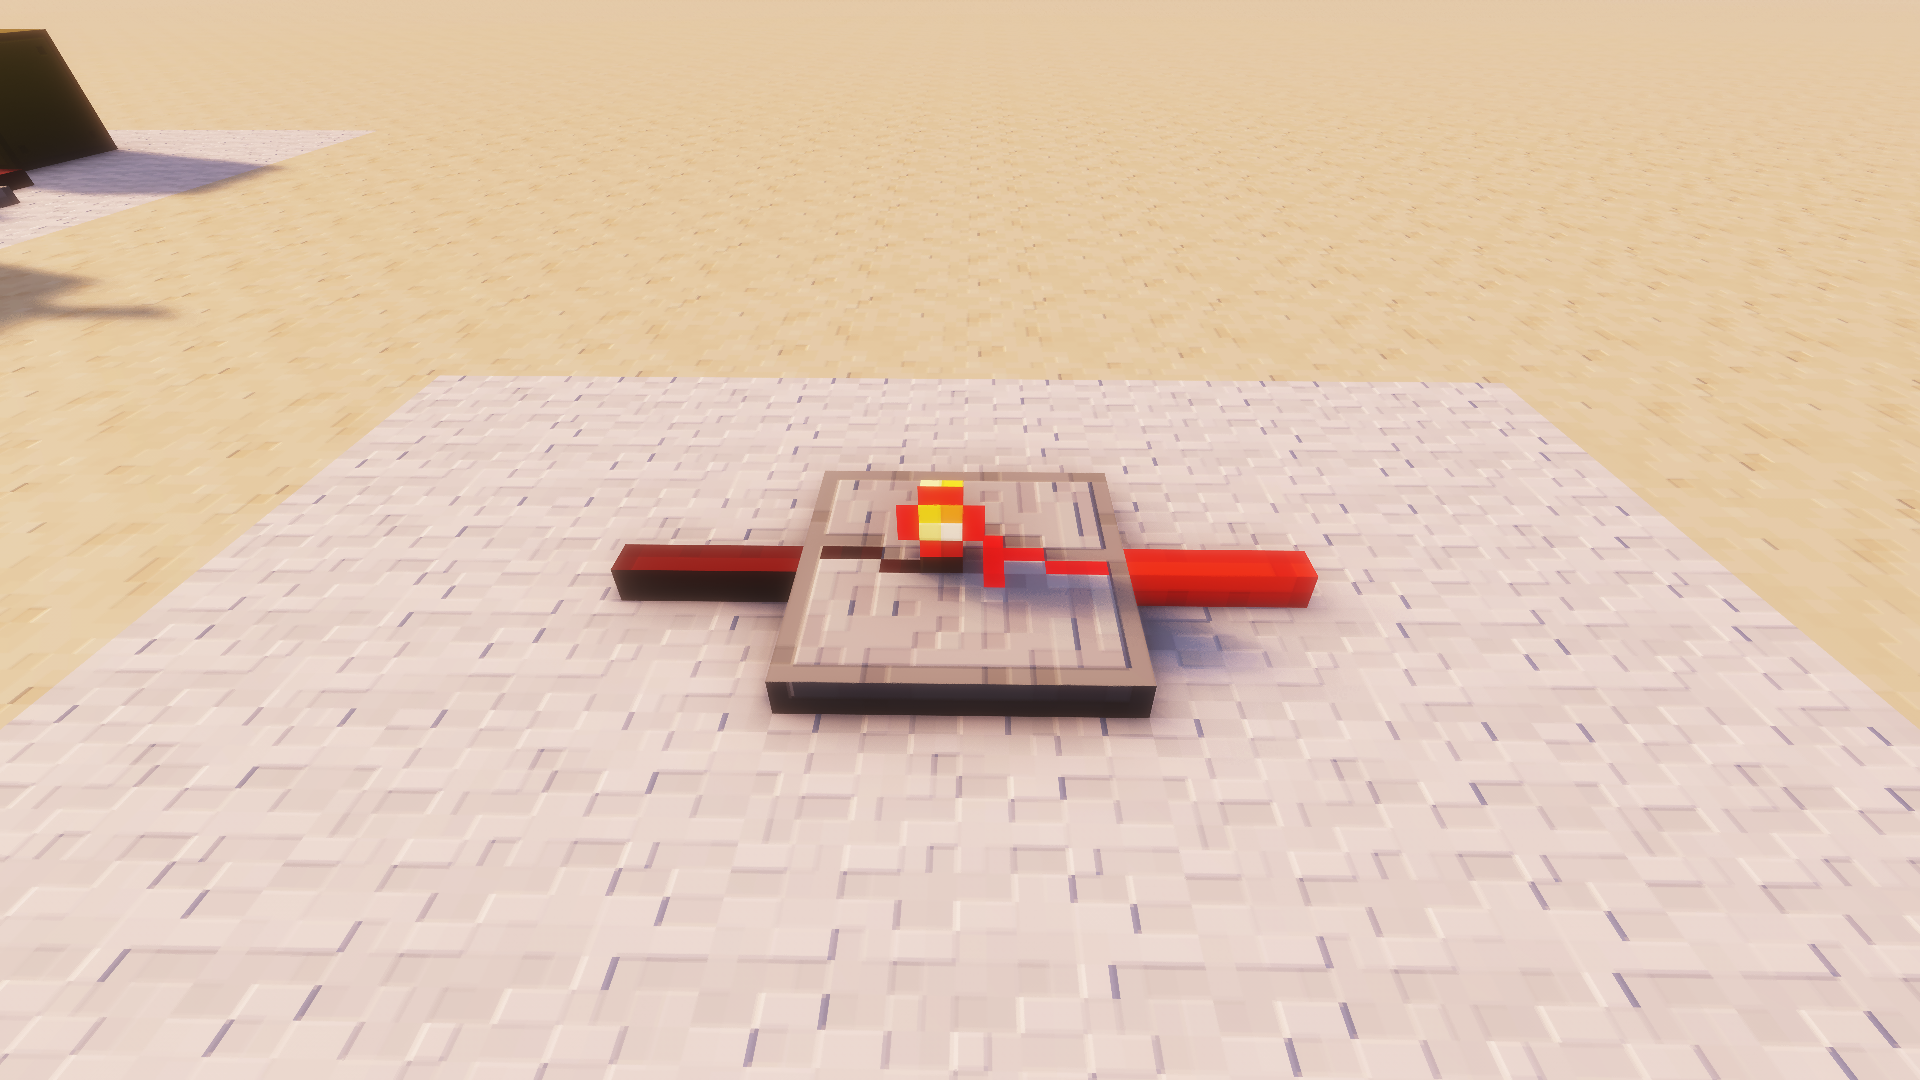
\includegraphics[width=0.7\linewidth]{images/not-wired-redstone.png}
    \caption{Porta Not de Redstone do mod Wired Redstone}
    \label{fig:not-wired-redstone}
\end{figure}

\subsubsection{And}

No jogo \textit{vanilla}, assim como na vida real, existem várias formas de se implementar o portão and. Entretanto, a forma mais utilizada no jogo é derivada da lei de De Morgan: 

\begin{center}
$(\lnot(p \land q) \equiv (\lnot p \lor \lnot q)) \iff ((p \land q) \equiv \lnot (\lnot p \lor \lnot q)) $
\end{center}

\begin{figure}[H]
    \centering
    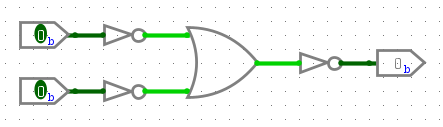
\includegraphics[width=0.7\linewidth]{images/and-circuit-alternative.png}
    \caption{Circuito alternativo para a porta And}
    \label{fig:and-circuit-alternative}
\end{figure}

\begin{figure}[H]
    \centering
    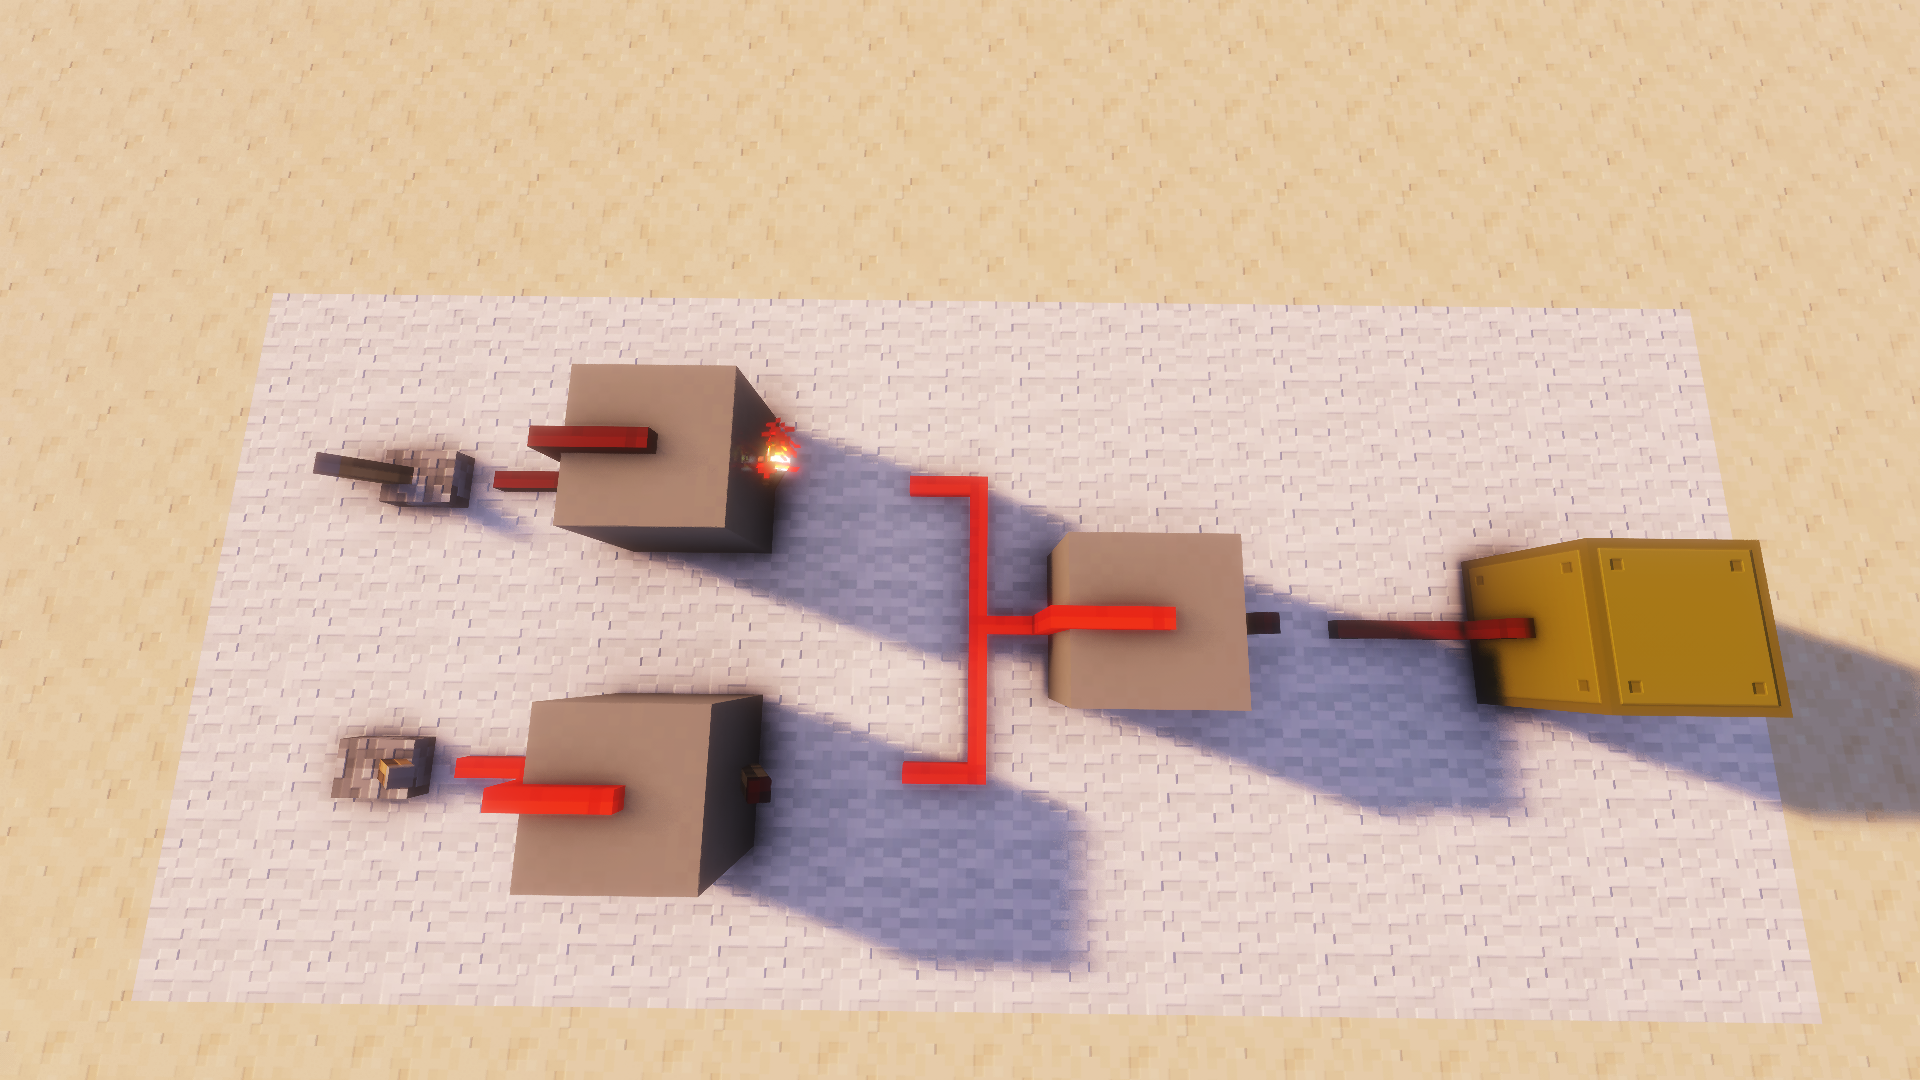
\includegraphics[width=0.7\linewidth]{images/and-redstone.png}
    \caption{Circuito And de Redstone para Minecraft Vanilla}
    \label{fig:and-redstone}
\end{figure}

\begin{figure}[H]
    \centering
    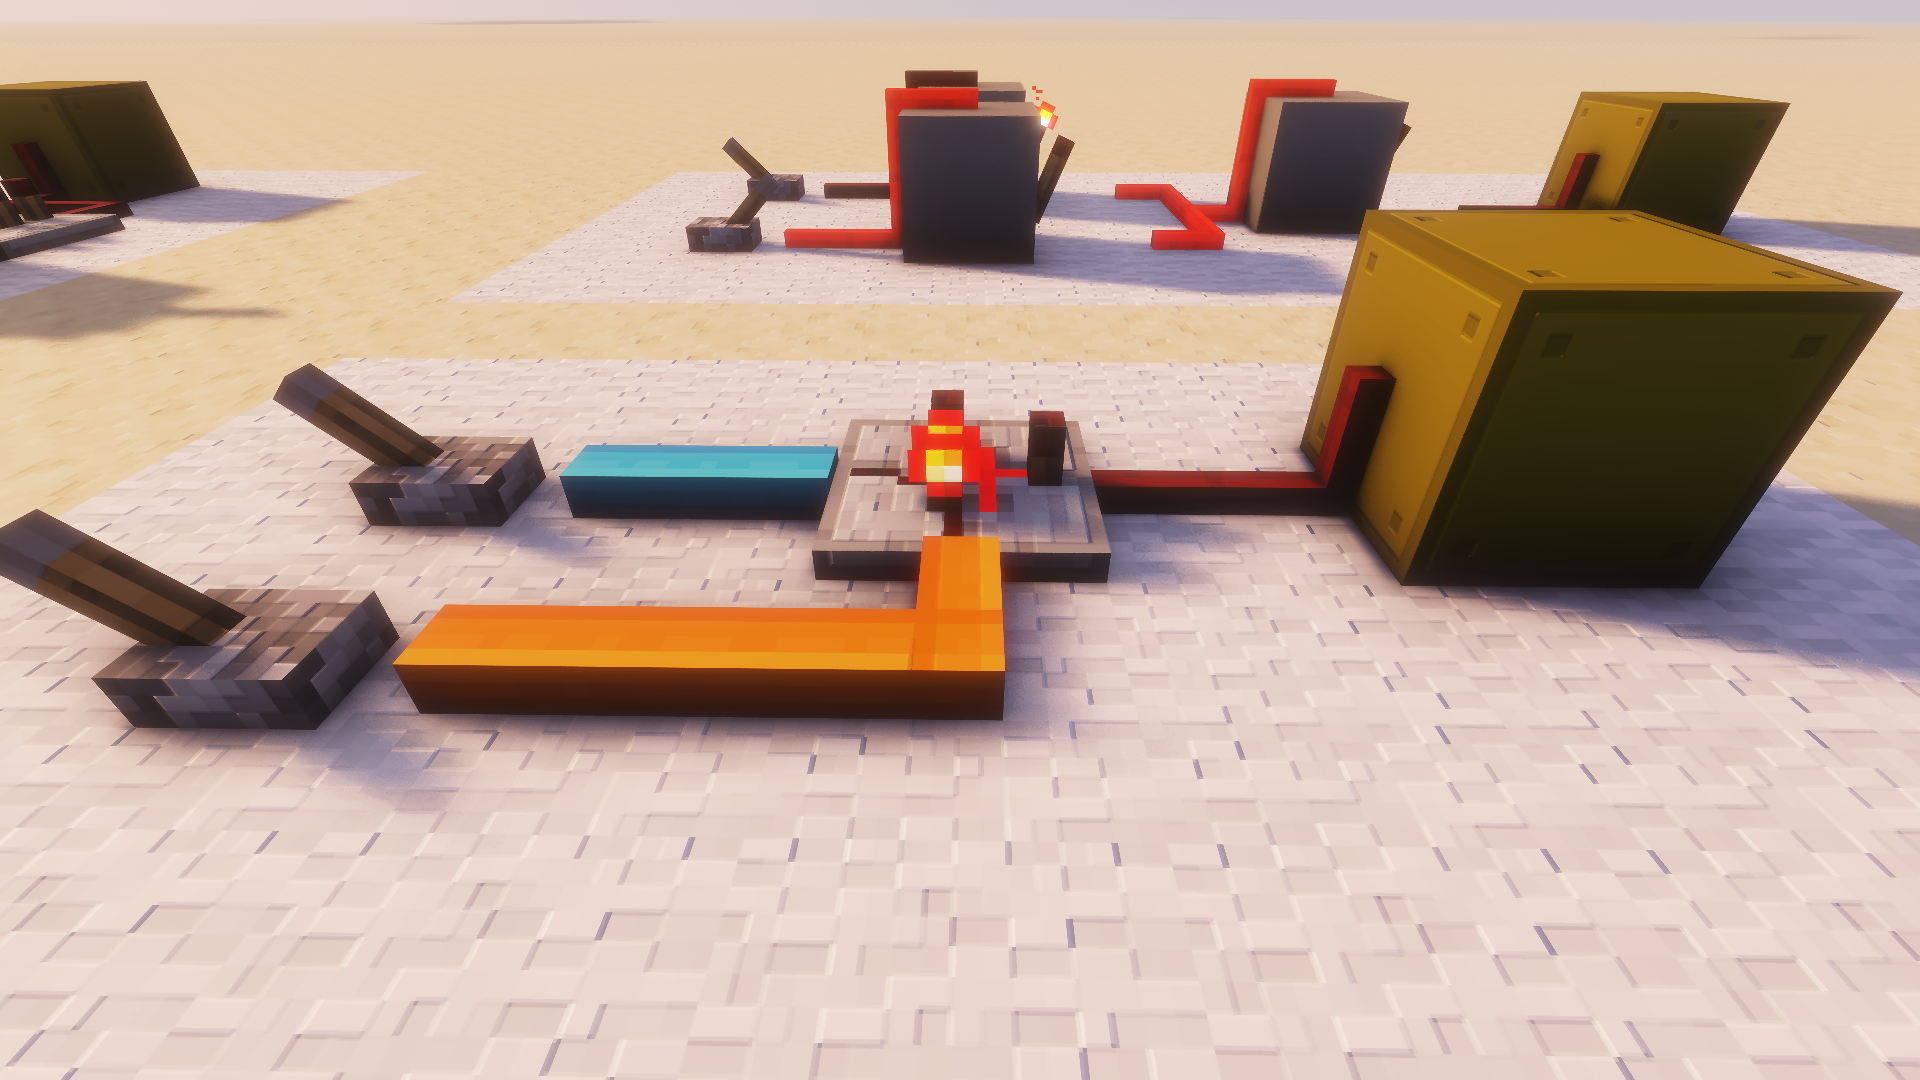
\includegraphics[width=0.7\linewidth]{images/and-wired-redstone.png}
    \caption{Circuito Integrado And Wired Redstone}
    \label{fig:and-wired-redstone}
\end{figure}

\subsubsection{Xor}

